\chapter{Transformada inversa de \emph{Fourier}}

\begin{equation}
    \mathcal{F}\{f(t)\}=F(\omega)
    \rightarrow
    \mathcal{F}^{-1}\{F(\omega)\}=f(t)
\end{equation}

Con la transformada inversa de \emph{Fourier} se regresa del dominio de
``$\omega$'' al dominio de ``$t$''.

\section{Tabla de transformadas de \emph{Fourier} inversas}

\begin{equation*}
\def\arraystretch{1.4}
\begin{array}{@{}cll@{}}
\toprule
 & F(\omega) & f(t)=\mathcal{F}^{-1}\{F(\omega)\}\\
\cmidrule(l){1-3}
 1 & \dfrac{1}{a+j\omega}
   & e^{-at}\,u(t)\quad\,a>0\\
\cmidrule(l){1-3}
 2 & \dfrac{1}{a-j\omega}
   & e^{at}\,u(-t)\quad\,a>0\\
\cmidrule(l){1-3}
 3 & \dfrac{2a}{a^2+\omega^2}
   & e^{-a|t|}\quad\,a>0\\
\cmidrule(l){1-3}
 4 & \frac{1}{\omega}\sen(a\omega)
   & \frac{1}{2}[u(t+a)-u(t-a)]\\
\cmidrule(l){1-3}
 5 & k
   & k\delta(t)\\
\cmidrule(l){1-3}
 6 & \dfrac{1}{\omega}
   & \frac{1}{2}j\,\sgn(t)\\
\bottomrule
\end{array}
\end{equation*}

\section{Propiedades de la transformada inversa de \emph{Fourier}}

\subsection{Linealidad}
\begin{equation}
    \mathcal{F}^{-1}\{a_1\,F_1(\omega)+a_2\,F_2(\omega)\}
    =a_1\,f_1(t)+a_2\,f_2(t)
\end{equation}

\subsection{Desplazamiento en $t$}
Si $\mathcal{F}^{-1}\{F(\omega)\}=f(t)$:
\begin{equation}
    \mathcal{F}^{-1}\{F(\omega)\,e^{-ja\omega}\}=f(t-a)
\end{equation}

\subsection{Desplazamiento en $\omega$}
Si $\mathcal{F}^{-1}\{F(\omega)\}=f(t)$:
\begin{equation}
    \mathcal{F}^{-1}\{F(\omega-a)\}=f(t)\,e^{jat}
\end{equation}

\section{Convolución}
Dadas dos funciones $f_1(t)$ y $f_2(t)$ definimos la convolución mediante la
siguiente integral:

\begin{equation}
    f(t)=f_1(t)*f_2(t)=\int_{-\infty}^{\infty}f_1(\tau)\,f_2(t-\tau)\,d\tau
\end{equation}

\begin{itemize}
    \item En $f_1(t)$ se reemplaza ``$t$'' por ``$\tau$'', permanece fija y no
    cambia.
    \item En $f_2(t)$ se reemplaza ``$t$'' por ``$t-\tau$''.La gráfica se
    refleja respecto al eje vertical, y luego se desplaza un ``$t$'' variable.
\end{itemize}

\begin{figure}[H]
    \centering
    \begin{minipage}{.4\textwidth}
        \centering
        % GNUPLOT: LaTeX picture with Postscript
\begingroup
  \makeatletter
  \providecommand\color[2][]{%
    \GenericError{(gnuplot) \space\space\space\@spaces}{%
      Package color not loaded in conjunction with
      terminal option `colourtext'%
    }{See the gnuplot documentation for explanation.%
    }{Either use 'blacktext' in gnuplot or load the package
      color.sty in LaTeX.}%
    \renewcommand\color[2][]{}%
  }%
  \providecommand\includegraphics[2][]{%
    \GenericError{(gnuplot) \space\space\space\@spaces}{%
      Package graphicx or graphics not loaded%
    }{See the gnuplot documentation for explanation.%
    }{The gnuplot epslatex terminal needs graphicx.sty or graphics.sty.}%
    \renewcommand\includegraphics[2][]{}%
  }%
  \providecommand\rotatebox[2]{#2}%
  \@ifundefined{ifGPcolor}{%
    \newif\ifGPcolor
    \GPcolorfalse
  }{}%
  \@ifundefined{ifGPblacktext}{%
    \newif\ifGPblacktext
    \GPblacktexttrue
  }{}%
  % define a \g@addto@macro without @ in the name:
  \let\gplgaddtomacro\g@addto@macro
  % define empty templates for all commands taking text:
  \gdef\gplbacktext{}%
  \gdef\gplfronttext{}%
  \makeatother
  \ifGPblacktext
    % no textcolor at all
    \def\colorrgb#1{}%
    \def\colorgray#1{}%
  \else
    % gray or color?
    \ifGPcolor
      \def\colorrgb#1{\color[rgb]{#1}}%
      \def\colorgray#1{\color[gray]{#1}}%
      \expandafter\def\csname LTw\endcsname{\color{white}}%
      \expandafter\def\csname LTb\endcsname{\color{black}}%
      \expandafter\def\csname LTa\endcsname{\color{black}}%
      \expandafter\def\csname LT0\endcsname{\color[rgb]{1,0,0}}%
      \expandafter\def\csname LT1\endcsname{\color[rgb]{0,1,0}}%
      \expandafter\def\csname LT2\endcsname{\color[rgb]{0,0,1}}%
      \expandafter\def\csname LT3\endcsname{\color[rgb]{1,0,1}}%
      \expandafter\def\csname LT4\endcsname{\color[rgb]{0,1,1}}%
      \expandafter\def\csname LT5\endcsname{\color[rgb]{1,1,0}}%
      \expandafter\def\csname LT6\endcsname{\color[rgb]{0,0,0}}%
      \expandafter\def\csname LT7\endcsname{\color[rgb]{1,0.3,0}}%
      \expandafter\def\csname LT8\endcsname{\color[rgb]{0.5,0.5,0.5}}%
    \else
      % gray
      \def\colorrgb#1{\color{black}}%
      \def\colorgray#1{\color[gray]{#1}}%
      \expandafter\def\csname LTw\endcsname{\color{white}}%
      \expandafter\def\csname LTb\endcsname{\color{black}}%
      \expandafter\def\csname LTa\endcsname{\color{black}}%
      \expandafter\def\csname LT0\endcsname{\color{black}}%
      \expandafter\def\csname LT1\endcsname{\color{black}}%
      \expandafter\def\csname LT2\endcsname{\color{black}}%
      \expandafter\def\csname LT3\endcsname{\color{black}}%
      \expandafter\def\csname LT4\endcsname{\color{black}}%
      \expandafter\def\csname LT5\endcsname{\color{black}}%
      \expandafter\def\csname LT6\endcsname{\color{black}}%
      \expandafter\def\csname LT7\endcsname{\color{black}}%
      \expandafter\def\csname LT8\endcsname{\color{black}}%
    \fi
  \fi
    \setlength{\unitlength}{0.0500bp}%
    \ifx\gptboxheight\undefined%
      \newlength{\gptboxheight}%
      \newlength{\gptboxwidth}%
      \newsavebox{\gptboxtext}%
    \fi%
    \setlength{\fboxrule}{0.5pt}%
    \setlength{\fboxsep}{1pt}%
    \definecolor{tbcol}{rgb}{1,1,1}%
\begin{picture}(3168.00,2160.00)%
    \gplgaddtomacro\gplbacktext{%
      \csname LTb\endcsname%%
      \put(1464,644){\makebox(0,0)[r]{\strut{}}}%
      \put(1464,1547){\makebox(0,0)[r]{\strut{}}}%
      \put(240,421){\makebox(0,0){\strut{}}}%
      \put(570,421){\makebox(0,0){\strut{}}}%
      \put(900,421){\makebox(0,0){\strut{}}}%
      \put(1230,421){\makebox(0,0){\strut{}}}%
      \put(1560,421){\makebox(0,0){\strut{}}}%
      \put(1889,421){\makebox(0,0){\strut{}}}%
      \put(2219,421){\makebox(0,0){\strut{}}}%
      \put(2549,421){\makebox(0,0){\strut{}}}%
      \put(2879,421){\makebox(0,0){\strut{}}}%
      \csname LTb\endcsname%%
      \put(3110,644){\makebox(0,0)[l]{\strut{}$t$}}%
      \put(1081,2270){\makebox(0,0)[l]{\strut{}$f(t)$}}%
      \put(2038,1999){\makebox(0,0)[l]{\strut{}$f_1(t)$}}%
      \put(1642,1276){\makebox(0,0)[l]{\strut{}$f_2(t)$}}%
    }%
    \gplgaddtomacro\gplfronttext{%
    }%
    \gplgaddtomacro\gplbacktext{%
      \csname LTb\endcsname%%
      \put(1464,644){\makebox(0,0)[r]{\strut{}}}%
      \put(1464,1547){\makebox(0,0)[r]{\strut{}}}%
      \put(240,421){\makebox(0,0){\strut{}}}%
      \put(570,421){\makebox(0,0){\strut{}}}%
      \put(900,421){\makebox(0,0){\strut{}}}%
      \put(1230,421){\makebox(0,0){\strut{}}}%
      \put(1560,421){\makebox(0,0){\strut{}}}%
      \put(1889,421){\makebox(0,0){\strut{}}}%
      \put(2219,421){\makebox(0,0){\strut{}}}%
      \put(2549,421){\makebox(0,0){\strut{}}}%
      \put(2879,421){\makebox(0,0){\strut{}}}%
      \csname LTb\endcsname%%
      \put(3110,644){\makebox(0,0)[l]{\strut{}$t$}}%
      \put(1081,2270){\makebox(0,0)[l]{\strut{}$f(t)$}}%
      \put(2038,1999){\makebox(0,0)[l]{\strut{}$f_1(t)$}}%
      \put(1642,1276){\makebox(0,0)[l]{\strut{}$f_2(t)$}}%
    }%
    \gplgaddtomacro\gplfronttext{%
    }%
    \gplbacktext
    \put(0,0){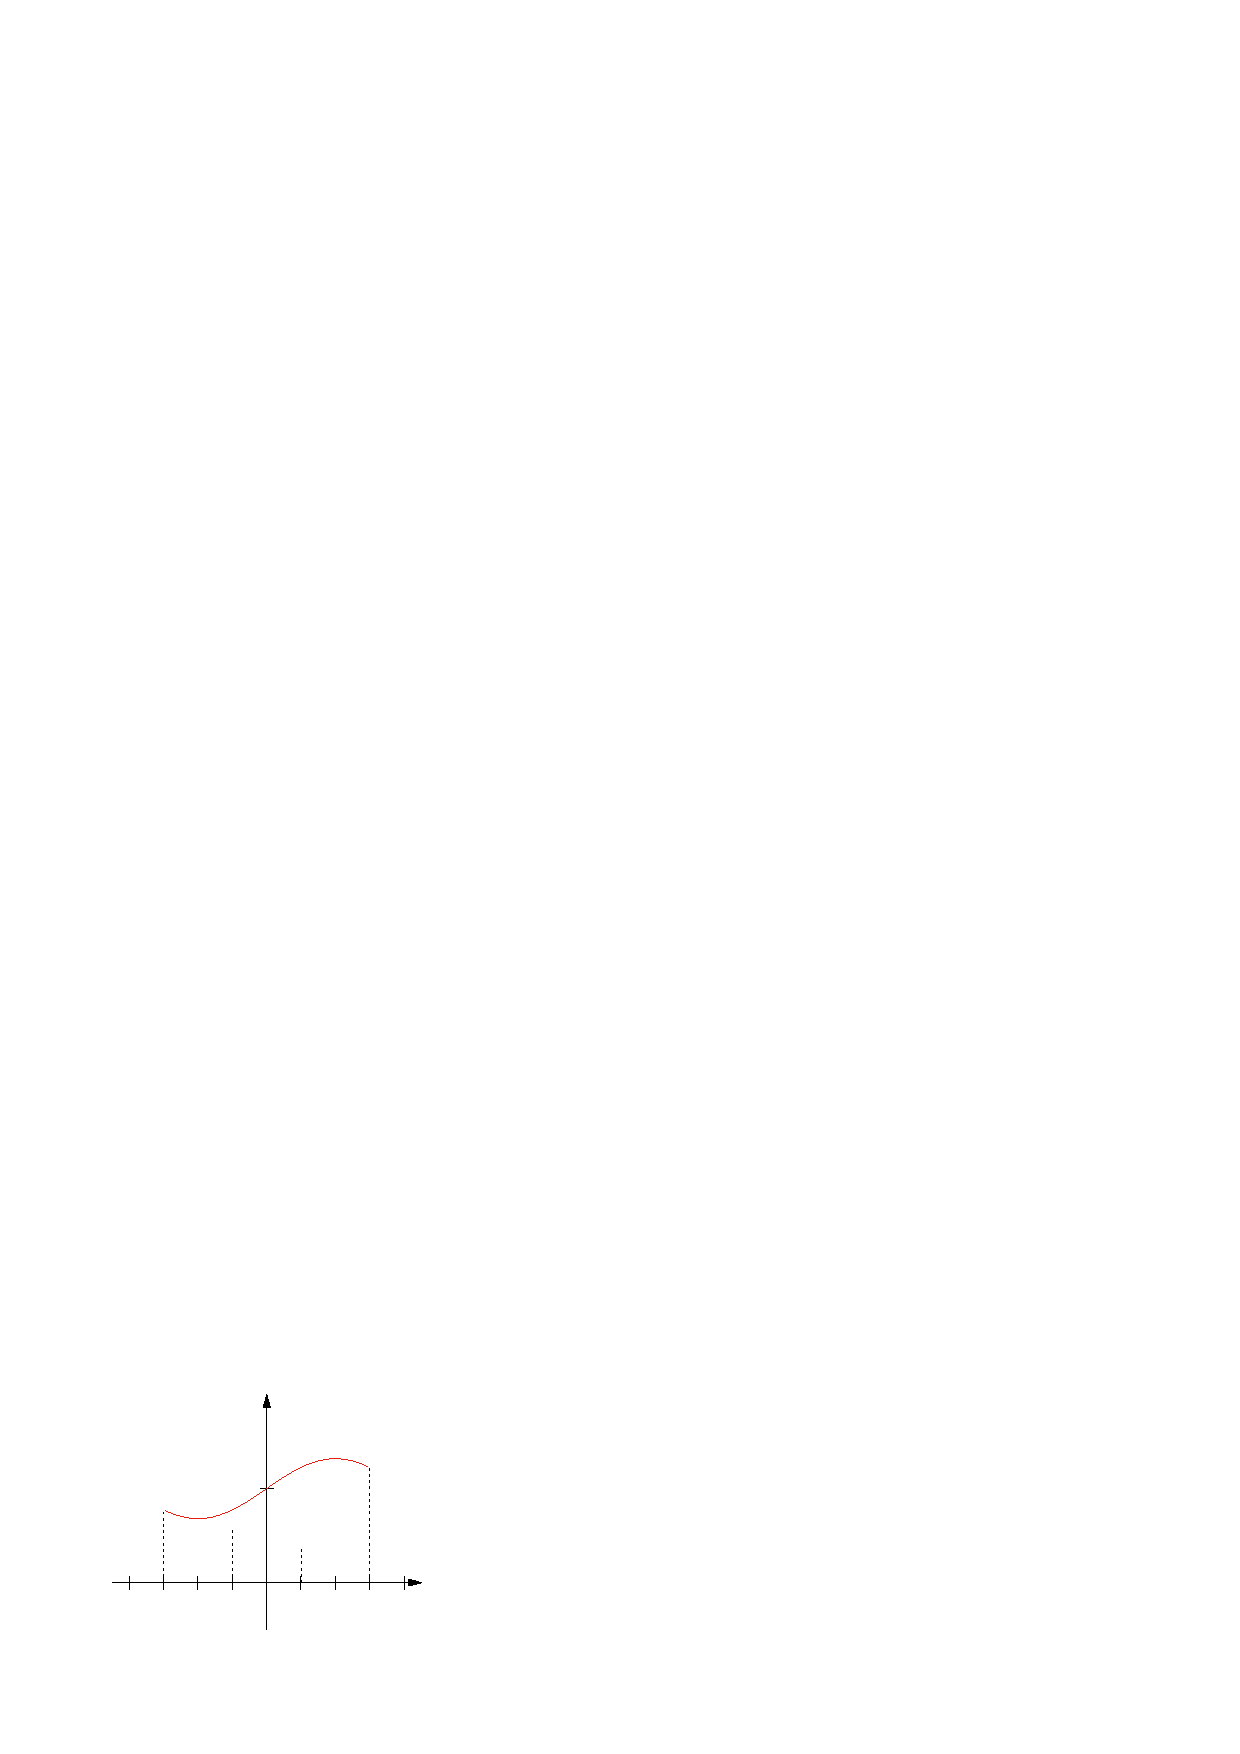
\includegraphics[width={158.40bp},height={108.00bp}]{figura_05_01}}%
    \gplfronttext
  \end{picture}%
\endgroup

    \end{minipage}
    \begin{minipage}{.4\textwidth}
        \centering
        % GNUPLOT: LaTeX picture with Postscript
\begingroup
  \makeatletter
  \providecommand\color[2][]{%
    \GenericError{(gnuplot) \space\space\space\@spaces}{%
      Package color not loaded in conjunction with
      terminal option `colourtext'%
    }{See the gnuplot documentation for explanation.%
    }{Either use 'blacktext' in gnuplot or load the package
      color.sty in LaTeX.}%
    \renewcommand\color[2][]{}%
  }%
  \providecommand\includegraphics[2][]{%
    \GenericError{(gnuplot) \space\space\space\@spaces}{%
      Package graphicx or graphics not loaded%
    }{See the gnuplot documentation for explanation.%
    }{The gnuplot epslatex terminal needs graphicx.sty or graphics.sty.}%
    \renewcommand\includegraphics[2][]{}%
  }%
  \providecommand\rotatebox[2]{#2}%
  \@ifundefined{ifGPcolor}{%
    \newif\ifGPcolor
    \GPcolorfalse
  }{}%
  \@ifundefined{ifGPblacktext}{%
    \newif\ifGPblacktext
    \GPblacktexttrue
  }{}%
  % define a \g@addto@macro without @ in the name:
  \let\gplgaddtomacro\g@addto@macro
  % define empty templates for all commands taking text:
  \gdef\gplbacktext{}%
  \gdef\gplfronttext{}%
  \makeatother
  \ifGPblacktext
    % no textcolor at all
    \def\colorrgb#1{}%
    \def\colorgray#1{}%
  \else
    % gray or color?
    \ifGPcolor
      \def\colorrgb#1{\color[rgb]{#1}}%
      \def\colorgray#1{\color[gray]{#1}}%
      \expandafter\def\csname LTw\endcsname{\color{white}}%
      \expandafter\def\csname LTb\endcsname{\color{black}}%
      \expandafter\def\csname LTa\endcsname{\color{black}}%
      \expandafter\def\csname LT0\endcsname{\color[rgb]{1,0,0}}%
      \expandafter\def\csname LT1\endcsname{\color[rgb]{0,1,0}}%
      \expandafter\def\csname LT2\endcsname{\color[rgb]{0,0,1}}%
      \expandafter\def\csname LT3\endcsname{\color[rgb]{1,0,1}}%
      \expandafter\def\csname LT4\endcsname{\color[rgb]{0,1,1}}%
      \expandafter\def\csname LT5\endcsname{\color[rgb]{1,1,0}}%
      \expandafter\def\csname LT6\endcsname{\color[rgb]{0,0,0}}%
      \expandafter\def\csname LT7\endcsname{\color[rgb]{1,0.3,0}}%
      \expandafter\def\csname LT8\endcsname{\color[rgb]{0.5,0.5,0.5}}%
    \else
      % gray
      \def\colorrgb#1{\color{black}}%
      \def\colorgray#1{\color[gray]{#1}}%
      \expandafter\def\csname LTw\endcsname{\color{white}}%
      \expandafter\def\csname LTb\endcsname{\color{black}}%
      \expandafter\def\csname LTa\endcsname{\color{black}}%
      \expandafter\def\csname LT0\endcsname{\color{black}}%
      \expandafter\def\csname LT1\endcsname{\color{black}}%
      \expandafter\def\csname LT2\endcsname{\color{black}}%
      \expandafter\def\csname LT3\endcsname{\color{black}}%
      \expandafter\def\csname LT4\endcsname{\color{black}}%
      \expandafter\def\csname LT5\endcsname{\color{black}}%
      \expandafter\def\csname LT6\endcsname{\color{black}}%
      \expandafter\def\csname LT7\endcsname{\color{black}}%
      \expandafter\def\csname LT8\endcsname{\color{black}}%
    \fi
  \fi
    \setlength{\unitlength}{0.0500bp}%
    \ifx\gptboxheight\undefined%
      \newlength{\gptboxheight}%
      \newlength{\gptboxwidth}%
      \newsavebox{\gptboxtext}%
    \fi%
    \setlength{\fboxrule}{0.5pt}%
    \setlength{\fboxsep}{1pt}%
    \definecolor{tbcol}{rgb}{1,1,1}%
\begin{picture}(3168.00,2160.00)%
    \gplgaddtomacro\gplbacktext{%
      \csname LTb\endcsname%%
      \put(1200,644){\makebox(0,0)[r]{\strut{}}}%
      \put(1200,1547){\makebox(0,0)[r]{\strut{}}}%
      \put(240,421){\makebox(0,0){\strut{}}}%
      \put(504,421){\makebox(0,0){\strut{}}}%
      \put(768,421){\makebox(0,0){\strut{}}}%
      \put(1032,421){\makebox(0,0){\strut{}}}%
      \put(1296,421){\makebox(0,0){\strut{}}}%
      \put(1560,421){\makebox(0,0){\strut{}}}%
      \put(1823,421){\makebox(0,0){\strut{}}}%
      \put(2087,421){\makebox(0,0){\strut{}}}%
      \put(2351,421){\makebox(0,0){\strut{}}}%
      \put(2615,421){\makebox(0,0){\strut{}}}%
      \put(2879,421){\makebox(0,0){\strut{}}}%
      \csname LTb\endcsname%%
      \put(3064,644){\makebox(0,0)[l]{\strut{}$t$}}%
      \put(834,2270){\makebox(0,0)[l]{\strut{}$f(\tau)$}}%
      \put(1678,1999){\makebox(0,0)[l]{\strut{}$f_1(\tau)$}}%
      \put(1084,1367){\makebox(0,0)[l]{\strut{}$f_2(-\tau)$}}%
      \put(2444,1367){\makebox(0,0)[l]{\strut{}$f_2(t-\tau)$}}%
      \put(1459,212){\makebox(0,0)[l]{\strut{}$t$}}%
    }%
    \gplgaddtomacro\gplfronttext{%
    }%
    \gplgaddtomacro\gplbacktext{%
      \csname LTb\endcsname%%
      \put(1200,644){\makebox(0,0)[r]{\strut{}}}%
      \put(1200,1547){\makebox(0,0)[r]{\strut{}}}%
      \put(240,421){\makebox(0,0){\strut{}}}%
      \put(504,421){\makebox(0,0){\strut{}}}%
      \put(768,421){\makebox(0,0){\strut{}}}%
      \put(1032,421){\makebox(0,0){\strut{}}}%
      \put(1296,421){\makebox(0,0){\strut{}}}%
      \put(1560,421){\makebox(0,0){\strut{}}}%
      \put(1823,421){\makebox(0,0){\strut{}}}%
      \put(2087,421){\makebox(0,0){\strut{}}}%
      \put(2351,421){\makebox(0,0){\strut{}}}%
      \put(2615,421){\makebox(0,0){\strut{}}}%
      \put(2879,421){\makebox(0,0){\strut{}}}%
      \csname LTb\endcsname%%
      \put(3064,644){\makebox(0,0)[l]{\strut{}$t$}}%
      \put(834,2270){\makebox(0,0)[l]{\strut{}$f(\tau)$}}%
      \put(1678,1999){\makebox(0,0)[l]{\strut{}$f_1(\tau)$}}%
      \put(1084,1367){\makebox(0,0)[l]{\strut{}$f_2(-\tau)$}}%
      \put(2444,1367){\makebox(0,0)[l]{\strut{}$f_2(t-\tau)$}}%
      \put(1459,212){\makebox(0,0)[l]{\strut{}$t$}}%
    }%
    \gplgaddtomacro\gplfronttext{%
    }%
    \gplgaddtomacro\gplbacktext{%
      \csname LTb\endcsname%%
      \put(1200,644){\makebox(0,0)[r]{\strut{}}}%
      \put(1200,1547){\makebox(0,0)[r]{\strut{}}}%
      \put(240,421){\makebox(0,0){\strut{}}}%
      \put(504,421){\makebox(0,0){\strut{}}}%
      \put(768,421){\makebox(0,0){\strut{}}}%
      \put(1032,421){\makebox(0,0){\strut{}}}%
      \put(1296,421){\makebox(0,0){\strut{}}}%
      \put(1560,421){\makebox(0,0){\strut{}}}%
      \put(1823,421){\makebox(0,0){\strut{}}}%
      \put(2087,421){\makebox(0,0){\strut{}}}%
      \put(2351,421){\makebox(0,0){\strut{}}}%
      \put(2615,421){\makebox(0,0){\strut{}}}%
      \put(2879,421){\makebox(0,0){\strut{}}}%
      \csname LTb\endcsname%%
      \put(3064,644){\makebox(0,0)[l]{\strut{}$t$}}%
      \put(834,2270){\makebox(0,0)[l]{\strut{}$f(\tau)$}}%
      \put(1678,1999){\makebox(0,0)[l]{\strut{}$f_1(\tau)$}}%
      \put(1084,1367){\makebox(0,0)[l]{\strut{}$f_2(-\tau)$}}%
      \put(2444,1367){\makebox(0,0)[l]{\strut{}$f_2(t-\tau)$}}%
      \put(1459,212){\makebox(0,0)[l]{\strut{}$t$}}%
    }%
    \gplgaddtomacro\gplfronttext{%
    }%
    \gplgaddtomacro\gplbacktext{%
      \csname LTb\endcsname%%
      \put(1200,644){\makebox(0,0)[r]{\strut{}}}%
      \put(1200,1547){\makebox(0,0)[r]{\strut{}}}%
      \put(240,421){\makebox(0,0){\strut{}}}%
      \put(504,421){\makebox(0,0){\strut{}}}%
      \put(768,421){\makebox(0,0){\strut{}}}%
      \put(1032,421){\makebox(0,0){\strut{}}}%
      \put(1296,421){\makebox(0,0){\strut{}}}%
      \put(1560,421){\makebox(0,0){\strut{}}}%
      \put(1823,421){\makebox(0,0){\strut{}}}%
      \put(2087,421){\makebox(0,0){\strut{}}}%
      \put(2351,421){\makebox(0,0){\strut{}}}%
      \put(2615,421){\makebox(0,0){\strut{}}}%
      \put(2879,421){\makebox(0,0){\strut{}}}%
      \csname LTb\endcsname%%
      \put(3064,644){\makebox(0,0)[l]{\strut{}$t$}}%
      \put(834,2270){\makebox(0,0)[l]{\strut{}$f(\tau)$}}%
      \put(1678,1999){\makebox(0,0)[l]{\strut{}$f_1(\tau)$}}%
      \put(1084,1367){\makebox(0,0)[l]{\strut{}$f_2(-\tau)$}}%
      \put(2444,1367){\makebox(0,0)[l]{\strut{}$f_2(t-\tau)$}}%
      \put(1459,212){\makebox(0,0)[l]{\strut{}$t$}}%
    }%
    \gplgaddtomacro\gplfronttext{%
    }%
    \gplgaddtomacro\gplbacktext{%
      \csname LTb\endcsname%%
      \put(1200,644){\makebox(0,0)[r]{\strut{}}}%
      \put(1200,1547){\makebox(0,0)[r]{\strut{}}}%
      \put(240,421){\makebox(0,0){\strut{}}}%
      \put(504,421){\makebox(0,0){\strut{}}}%
      \put(768,421){\makebox(0,0){\strut{}}}%
      \put(1032,421){\makebox(0,0){\strut{}}}%
      \put(1296,421){\makebox(0,0){\strut{}}}%
      \put(1560,421){\makebox(0,0){\strut{}}}%
      \put(1823,421){\makebox(0,0){\strut{}}}%
      \put(2087,421){\makebox(0,0){\strut{}}}%
      \put(2351,421){\makebox(0,0){\strut{}}}%
      \put(2615,421){\makebox(0,0){\strut{}}}%
      \put(2879,421){\makebox(0,0){\strut{}}}%
      \csname LTb\endcsname%%
      \put(3064,644){\makebox(0,0)[l]{\strut{}$t$}}%
      \put(834,2270){\makebox(0,0)[l]{\strut{}$f(\tau)$}}%
      \put(1678,1999){\makebox(0,0)[l]{\strut{}$f_1(\tau)$}}%
      \put(1084,1367){\makebox(0,0)[l]{\strut{}$f_2(-\tau)$}}%
      \put(2444,1367){\makebox(0,0)[l]{\strut{}$f_2(t-\tau)$}}%
      \put(1459,212){\makebox(0,0)[l]{\strut{}$t$}}%
    }%
    \gplgaddtomacro\gplfronttext{%
    }%
    \gplbacktext
    \put(0,0){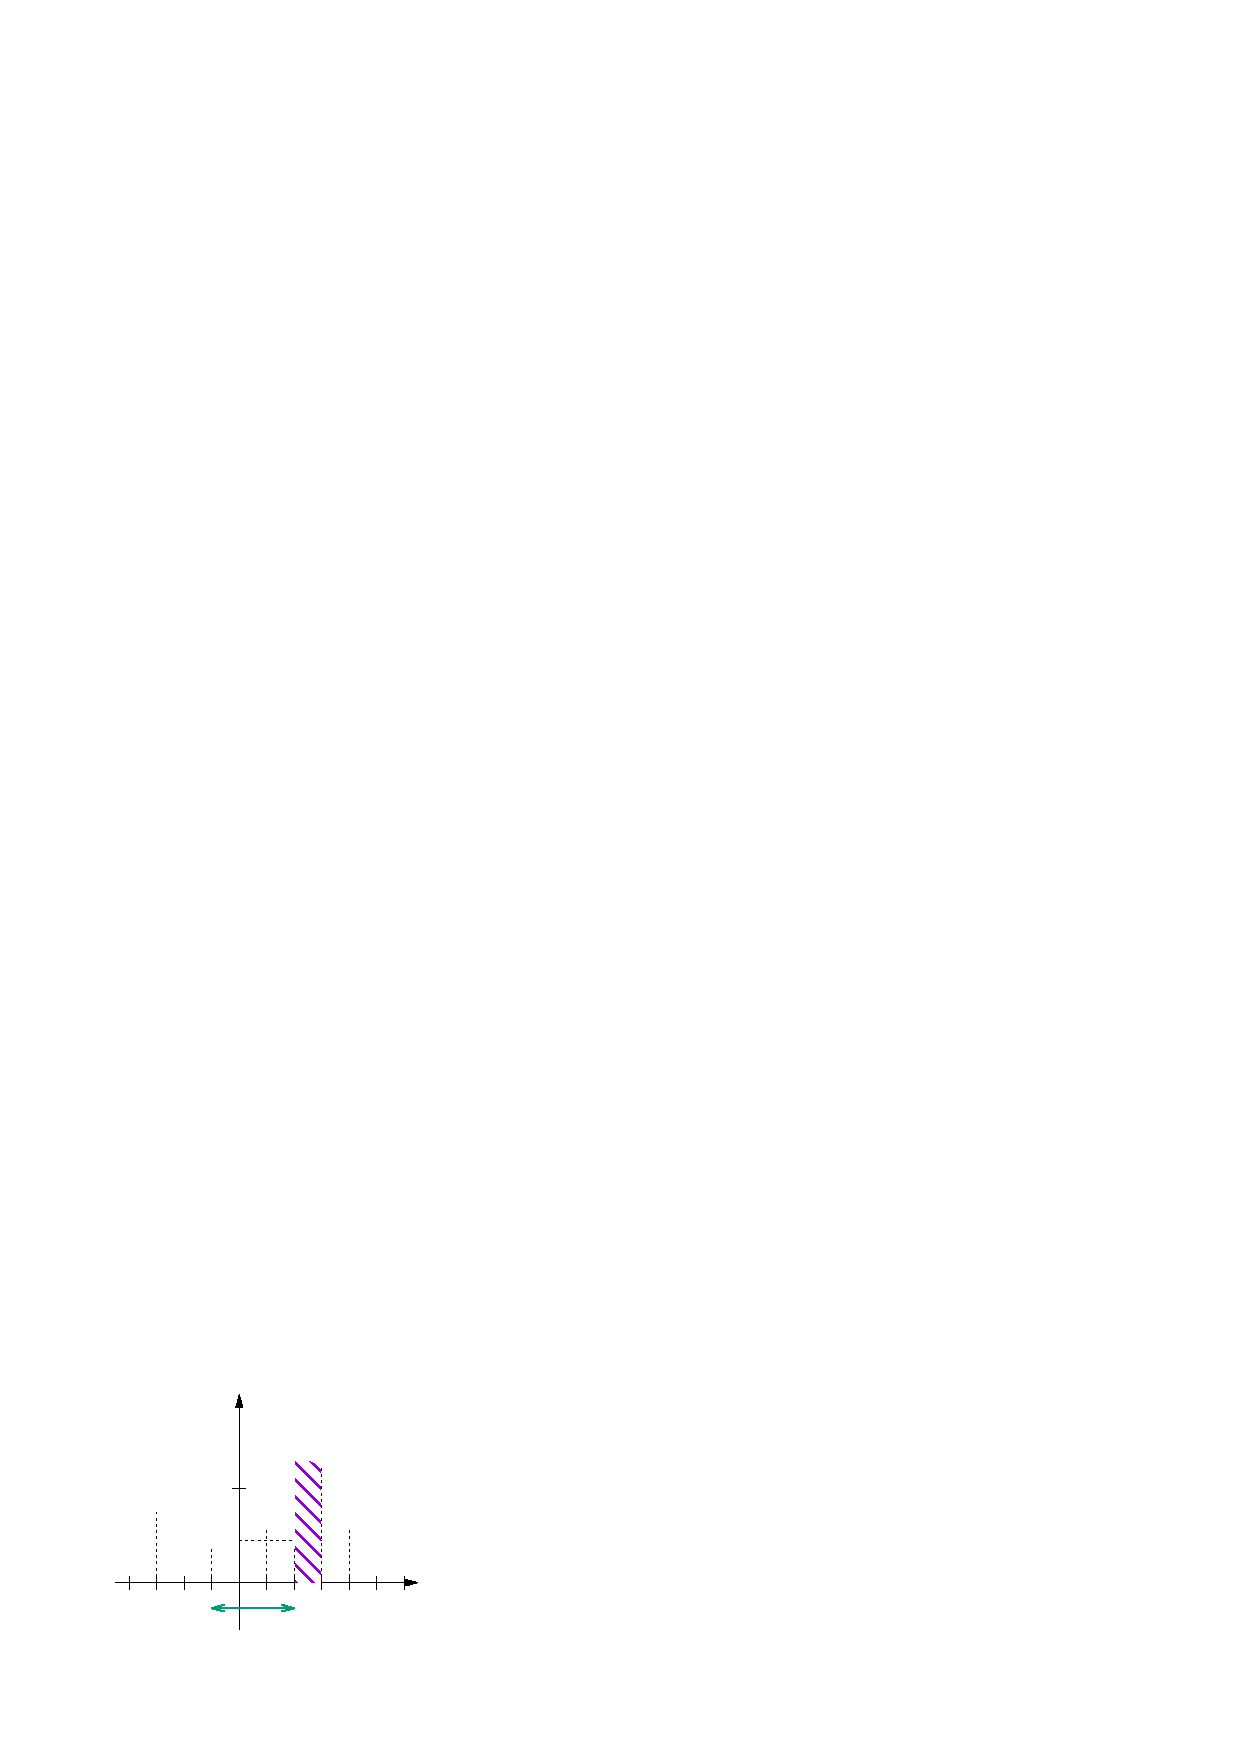
\includegraphics[width={158.40bp},height={108.00bp}]{figura_05_02}}%
    \gplfronttext
  \end{picture}%
\endgroup

    \end{minipage}
\end{figure}
El intervalo de integración será el intervalo donde ambas gráficas se
superponen.

\section{Propiedades de la convolución}

\subsection{Conmutatividad}
\begin{equation}
    f_1(t)*f_2(t)=f_2(t)*f_1(t)
\end{equation}

\subsection{Asociatividad}
\begin{equation}
    f_1(t)*[f_2(t)*f_3(t)]=[f_1(t)*f_2(t)]*f_3(t)
\end{equation}

\subsection{Distributividad}
\begin{equation}
    f_1(t)*[f_2(t)+f_3(t)]=f_1(t)*f_2(t)+f_1(t)*f_3(t)
\end{equation}

\subsection{Función impulso}
\begin{equation}
    f_1(t)*\delta(t-t_0)=f_1(t-t_0)
\end{equation}

\underline{Prueba}:

\begin{equation*}
    f_1(t)*\delta(t-t_0)
    =\int_{-\infty}^{\infty}\,f_1(t-\tau)\,\delta(\tau-t_0)\,d\tau
    =f_1(t-t_0)
\end{equation*}

\subsection{Función escalón unitario}
Si $f_1(t)=f_1(t)\,u(t)$ y $f_2(t)=f_2(t)\,u(t)$:
\begin{equation}
    f_1(t)*f_2(t)=\int_0^t\,f_1(\tau)\,f_2(t-\tau)\,d\tau
\end{equation}

\begin{figure}[H]
    \centering
    \begin{minipage}{.4\textwidth}
        \centering
        % GNUPLOT: LaTeX picture with Postscript
\begingroup
  \makeatletter
  \providecommand\color[2][]{%
    \GenericError{(gnuplot) \space\space\space\@spaces}{%
      Package color not loaded in conjunction with
      terminal option `colourtext'%
    }{See the gnuplot documentation for explanation.%
    }{Either use 'blacktext' in gnuplot or load the package
      color.sty in LaTeX.}%
    \renewcommand\color[2][]{}%
  }%
  \providecommand\includegraphics[2][]{%
    \GenericError{(gnuplot) \space\space\space\@spaces}{%
      Package graphicx or graphics not loaded%
    }{See the gnuplot documentation for explanation.%
    }{The gnuplot epslatex terminal needs graphicx.sty or graphics.sty.}%
    \renewcommand\includegraphics[2][]{}%
  }%
  \providecommand\rotatebox[2]{#2}%
  \@ifundefined{ifGPcolor}{%
    \newif\ifGPcolor
    \GPcolorfalse
  }{}%
  \@ifundefined{ifGPblacktext}{%
    \newif\ifGPblacktext
    \GPblacktexttrue
  }{}%
  % define a \g@addto@macro without @ in the name:
  \let\gplgaddtomacro\g@addto@macro
  % define empty templates for all commands taking text:
  \gdef\gplbacktext{}%
  \gdef\gplfronttext{}%
  \makeatother
  \ifGPblacktext
    % no textcolor at all
    \def\colorrgb#1{}%
    \def\colorgray#1{}%
  \else
    % gray or color?
    \ifGPcolor
      \def\colorrgb#1{\color[rgb]{#1}}%
      \def\colorgray#1{\color[gray]{#1}}%
      \expandafter\def\csname LTw\endcsname{\color{white}}%
      \expandafter\def\csname LTb\endcsname{\color{black}}%
      \expandafter\def\csname LTa\endcsname{\color{black}}%
      \expandafter\def\csname LT0\endcsname{\color[rgb]{1,0,0}}%
      \expandafter\def\csname LT1\endcsname{\color[rgb]{0,1,0}}%
      \expandafter\def\csname LT2\endcsname{\color[rgb]{0,0,1}}%
      \expandafter\def\csname LT3\endcsname{\color[rgb]{1,0,1}}%
      \expandafter\def\csname LT4\endcsname{\color[rgb]{0,1,1}}%
      \expandafter\def\csname LT5\endcsname{\color[rgb]{1,1,0}}%
      \expandafter\def\csname LT6\endcsname{\color[rgb]{0,0,0}}%
      \expandafter\def\csname LT7\endcsname{\color[rgb]{1,0.3,0}}%
      \expandafter\def\csname LT8\endcsname{\color[rgb]{0.5,0.5,0.5}}%
    \else
      % gray
      \def\colorrgb#1{\color{black}}%
      \def\colorgray#1{\color[gray]{#1}}%
      \expandafter\def\csname LTw\endcsname{\color{white}}%
      \expandafter\def\csname LTb\endcsname{\color{black}}%
      \expandafter\def\csname LTa\endcsname{\color{black}}%
      \expandafter\def\csname LT0\endcsname{\color{black}}%
      \expandafter\def\csname LT1\endcsname{\color{black}}%
      \expandafter\def\csname LT2\endcsname{\color{black}}%
      \expandafter\def\csname LT3\endcsname{\color{black}}%
      \expandafter\def\csname LT4\endcsname{\color{black}}%
      \expandafter\def\csname LT5\endcsname{\color{black}}%
      \expandafter\def\csname LT6\endcsname{\color{black}}%
      \expandafter\def\csname LT7\endcsname{\color{black}}%
      \expandafter\def\csname LT8\endcsname{\color{black}}%
    \fi
  \fi
    \setlength{\unitlength}{0.0500bp}%
    \ifx\gptboxheight\undefined%
      \newlength{\gptboxheight}%
      \newlength{\gptboxwidth}%
      \newsavebox{\gptboxtext}%
    \fi%
    \setlength{\fboxrule}{0.5pt}%
    \setlength{\fboxsep}{1pt}%
    \definecolor{tbcol}{rgb}{1,1,1}%
\begin{picture}(3168.00,2160.00)%
    \gplgaddtomacro\gplbacktext{%
      \csname LTb\endcsname%%
      \put(437,644){\makebox(0,0)[r]{\strut{}}}%
      \put(437,1547){\makebox(0,0)[r]{\strut{}}}%
      \put(533,421){\makebox(0,0){\strut{}}}%
      \put(1120,421){\makebox(0,0){\strut{}}}%
      \put(1706,421){\makebox(0,0){\strut{}}}%
      \put(2293,421){\makebox(0,0){\strut{}}}%
      \put(2879,421){\makebox(0,0){\strut{}}}%
      \csname LTb\endcsname%%
      \put(3290,644){\makebox(0,0)[l]{\strut{}$t$}}%
      \put(5,2360){\makebox(0,0)[l]{\strut{}$f(t)$}}%
      \put(1384,1999){\makebox(0,0)[l]{\strut{}$f_1(t)$}}%
      \put(1120,1276){\makebox(0,0)[l]{\strut{}$f_2(t)$}}%
    }%
    \gplgaddtomacro\gplfronttext{%
    }%
    \gplgaddtomacro\gplbacktext{%
      \csname LTb\endcsname%%
      \put(437,644){\makebox(0,0)[r]{\strut{}}}%
      \put(437,1547){\makebox(0,0)[r]{\strut{}}}%
      \put(533,421){\makebox(0,0){\strut{}}}%
      \put(1120,421){\makebox(0,0){\strut{}}}%
      \put(1706,421){\makebox(0,0){\strut{}}}%
      \put(2293,421){\makebox(0,0){\strut{}}}%
      \put(2879,421){\makebox(0,0){\strut{}}}%
      \csname LTb\endcsname%%
      \put(3290,644){\makebox(0,0)[l]{\strut{}$t$}}%
      \put(5,2360){\makebox(0,0)[l]{\strut{}$f(t)$}}%
      \put(1384,1999){\makebox(0,0)[l]{\strut{}$f_1(t)$}}%
      \put(1120,1276){\makebox(0,0)[l]{\strut{}$f_2(t)$}}%
    }%
    \gplgaddtomacro\gplfronttext{%
    }%
    \gplbacktext
    \put(0,0){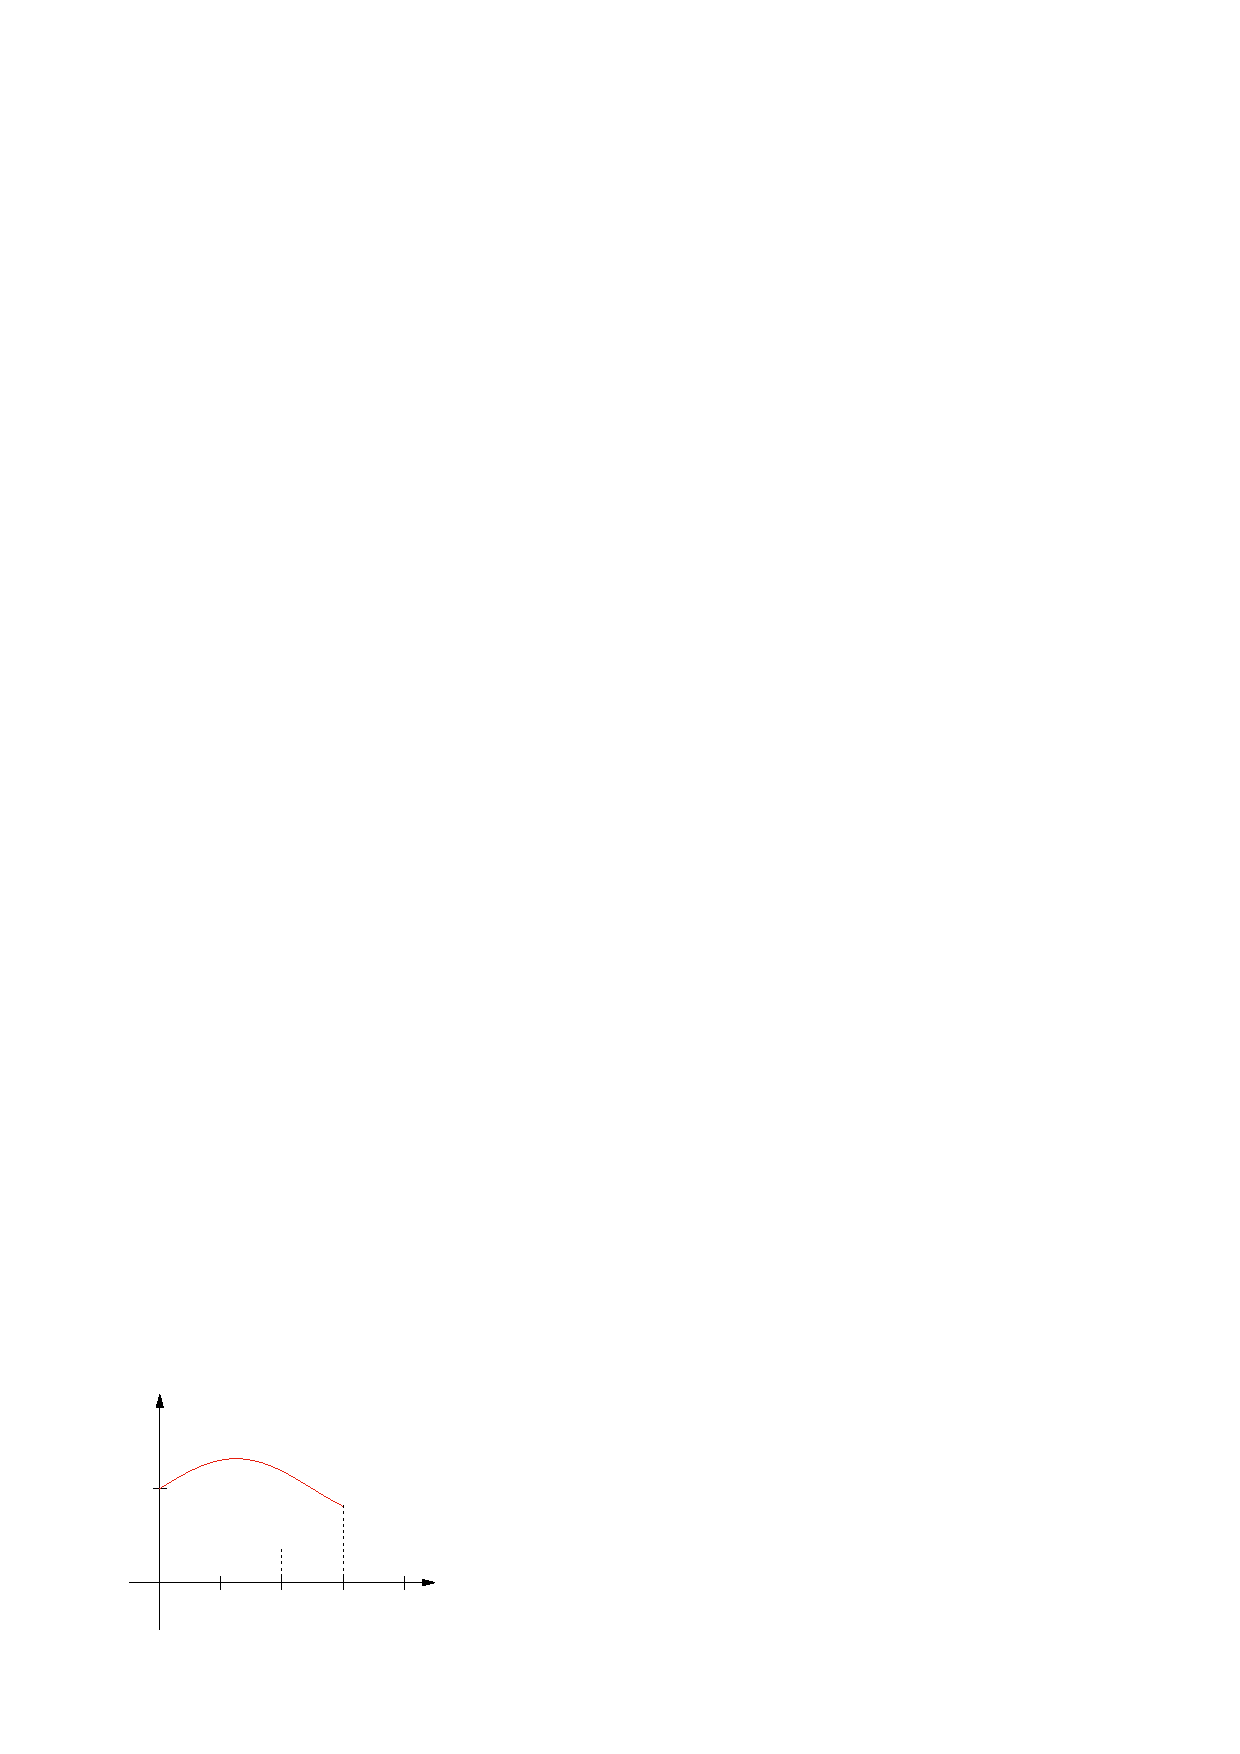
\includegraphics[width={158.40bp},height={108.00bp}]{figura_05_03}}%
    \gplfronttext
  \end{picture}%
\endgroup

    \end{minipage}
    \begin{minipage}{.4\textwidth}
        \centering
        % GNUPLOT: LaTeX picture with Postscript
\begingroup
  \makeatletter
  \providecommand\color[2][]{%
    \GenericError{(gnuplot) \space\space\space\@spaces}{%
      Package color not loaded in conjunction with
      terminal option `colourtext'%
    }{See the gnuplot documentation for explanation.%
    }{Either use 'blacktext' in gnuplot or load the package
      color.sty in LaTeX.}%
    \renewcommand\color[2][]{}%
  }%
  \providecommand\includegraphics[2][]{%
    \GenericError{(gnuplot) \space\space\space\@spaces}{%
      Package graphicx or graphics not loaded%
    }{See the gnuplot documentation for explanation.%
    }{The gnuplot epslatex terminal needs graphicx.sty or graphics.sty.}%
    \renewcommand\includegraphics[2][]{}%
  }%
  \providecommand\rotatebox[2]{#2}%
  \@ifundefined{ifGPcolor}{%
    \newif\ifGPcolor
    \GPcolorfalse
  }{}%
  \@ifundefined{ifGPblacktext}{%
    \newif\ifGPblacktext
    \GPblacktexttrue
  }{}%
  % define a \g@addto@macro without @ in the name:
  \let\gplgaddtomacro\g@addto@macro
  % define empty templates for all commands taking text:
  \gdef\gplbacktext{}%
  \gdef\gplfronttext{}%
  \makeatother
  \ifGPblacktext
    % no textcolor at all
    \def\colorrgb#1{}%
    \def\colorgray#1{}%
  \else
    % gray or color?
    \ifGPcolor
      \def\colorrgb#1{\color[rgb]{#1}}%
      \def\colorgray#1{\color[gray]{#1}}%
      \expandafter\def\csname LTw\endcsname{\color{white}}%
      \expandafter\def\csname LTb\endcsname{\color{black}}%
      \expandafter\def\csname LTa\endcsname{\color{black}}%
      \expandafter\def\csname LT0\endcsname{\color[rgb]{1,0,0}}%
      \expandafter\def\csname LT1\endcsname{\color[rgb]{0,1,0}}%
      \expandafter\def\csname LT2\endcsname{\color[rgb]{0,0,1}}%
      \expandafter\def\csname LT3\endcsname{\color[rgb]{1,0,1}}%
      \expandafter\def\csname LT4\endcsname{\color[rgb]{0,1,1}}%
      \expandafter\def\csname LT5\endcsname{\color[rgb]{1,1,0}}%
      \expandafter\def\csname LT6\endcsname{\color[rgb]{0,0,0}}%
      \expandafter\def\csname LT7\endcsname{\color[rgb]{1,0.3,0}}%
      \expandafter\def\csname LT8\endcsname{\color[rgb]{0.5,0.5,0.5}}%
    \else
      % gray
      \def\colorrgb#1{\color{black}}%
      \def\colorgray#1{\color[gray]{#1}}%
      \expandafter\def\csname LTw\endcsname{\color{white}}%
      \expandafter\def\csname LTb\endcsname{\color{black}}%
      \expandafter\def\csname LTa\endcsname{\color{black}}%
      \expandafter\def\csname LT0\endcsname{\color{black}}%
      \expandafter\def\csname LT1\endcsname{\color{black}}%
      \expandafter\def\csname LT2\endcsname{\color{black}}%
      \expandafter\def\csname LT3\endcsname{\color{black}}%
      \expandafter\def\csname LT4\endcsname{\color{black}}%
      \expandafter\def\csname LT5\endcsname{\color{black}}%
      \expandafter\def\csname LT6\endcsname{\color{black}}%
      \expandafter\def\csname LT7\endcsname{\color{black}}%
      \expandafter\def\csname LT8\endcsname{\color{black}}%
    \fi
  \fi
    \setlength{\unitlength}{0.0500bp}%
    \ifx\gptboxheight\undefined%
      \newlength{\gptboxheight}%
      \newlength{\gptboxwidth}%
      \newsavebox{\gptboxtext}%
    \fi%
    \setlength{\fboxrule}{0.5pt}%
    \setlength{\fboxsep}{1pt}%
    \definecolor{tbcol}{rgb}{1,1,1}%
\begin{picture}(3168.00,2160.00)%
    \gplgaddtomacro\gplbacktext{%
      \csname LTb\endcsname%%
      \put(437,644){\makebox(0,0)[r]{\strut{}}}%
      \put(437,1547){\makebox(0,0)[r]{\strut{}}}%
      \put(533,421){\makebox(0,0){\strut{}}}%
      \put(1120,421){\makebox(0,0){\strut{}}}%
      \put(1706,421){\makebox(0,0){\strut{}}}%
      \put(2293,421){\makebox(0,0){\strut{}}}%
      \put(2879,421){\makebox(0,0){\strut{}}}%
      \csname LTb\endcsname%%
      \put(3290,644){\makebox(0,0)[l]{\strut{}$t$}}%
      \put(5,2360){\makebox(0,0)[l]{\strut{}$f(\tau)$}}%
      \put(1384,1999){\makebox(0,0)[l]{\strut{}$f_1(\tau)$}}%
      \put(1237,1276){\makebox(0,0)[l]{\strut{}$f_2(t-\tau)$}}%
      \put(1061,428){\makebox(0,0)[l]{\strut{}$t$}}%
    }%
    \gplgaddtomacro\gplfronttext{%
    }%
    \gplgaddtomacro\gplbacktext{%
      \csname LTb\endcsname%%
      \put(437,644){\makebox(0,0)[r]{\strut{}}}%
      \put(437,1547){\makebox(0,0)[r]{\strut{}}}%
      \put(533,421){\makebox(0,0){\strut{}}}%
      \put(1120,421){\makebox(0,0){\strut{}}}%
      \put(1706,421){\makebox(0,0){\strut{}}}%
      \put(2293,421){\makebox(0,0){\strut{}}}%
      \put(2879,421){\makebox(0,0){\strut{}}}%
      \csname LTb\endcsname%%
      \put(3290,644){\makebox(0,0)[l]{\strut{}$t$}}%
      \put(5,2360){\makebox(0,0)[l]{\strut{}$f(\tau)$}}%
      \put(1384,1999){\makebox(0,0)[l]{\strut{}$f_1(\tau)$}}%
      \put(1237,1276){\makebox(0,0)[l]{\strut{}$f_2(t-\tau)$}}%
      \put(1061,428){\makebox(0,0)[l]{\strut{}$t$}}%
    }%
    \gplgaddtomacro\gplfronttext{%
    }%
    \gplgaddtomacro\gplbacktext{%
      \csname LTb\endcsname%%
      \put(437,644){\makebox(0,0)[r]{\strut{}}}%
      \put(437,1547){\makebox(0,0)[r]{\strut{}}}%
      \put(533,421){\makebox(0,0){\strut{}}}%
      \put(1120,421){\makebox(0,0){\strut{}}}%
      \put(1706,421){\makebox(0,0){\strut{}}}%
      \put(2293,421){\makebox(0,0){\strut{}}}%
      \put(2879,421){\makebox(0,0){\strut{}}}%
      \csname LTb\endcsname%%
      \put(3290,644){\makebox(0,0)[l]{\strut{}$t$}}%
      \put(5,2360){\makebox(0,0)[l]{\strut{}$f(\tau)$}}%
      \put(1384,1999){\makebox(0,0)[l]{\strut{}$f_1(\tau)$}}%
      \put(1237,1276){\makebox(0,0)[l]{\strut{}$f_2(t-\tau)$}}%
      \put(1061,428){\makebox(0,0)[l]{\strut{}$t$}}%
    }%
    \gplgaddtomacro\gplfronttext{%
    }%
    \gplgaddtomacro\gplbacktext{%
      \csname LTb\endcsname%%
      \put(437,644){\makebox(0,0)[r]{\strut{}}}%
      \put(437,1547){\makebox(0,0)[r]{\strut{}}}%
      \put(533,421){\makebox(0,0){\strut{}}}%
      \put(1120,421){\makebox(0,0){\strut{}}}%
      \put(1706,421){\makebox(0,0){\strut{}}}%
      \put(2293,421){\makebox(0,0){\strut{}}}%
      \put(2879,421){\makebox(0,0){\strut{}}}%
      \csname LTb\endcsname%%
      \put(3290,644){\makebox(0,0)[l]{\strut{}$t$}}%
      \put(5,2360){\makebox(0,0)[l]{\strut{}$f(\tau)$}}%
      \put(1384,1999){\makebox(0,0)[l]{\strut{}$f_1(\tau)$}}%
      \put(1237,1276){\makebox(0,0)[l]{\strut{}$f_2(t-\tau)$}}%
      \put(1061,428){\makebox(0,0)[l]{\strut{}$t$}}%
    }%
    \gplgaddtomacro\gplfronttext{%
    }%
    \gplbacktext
    \put(0,0){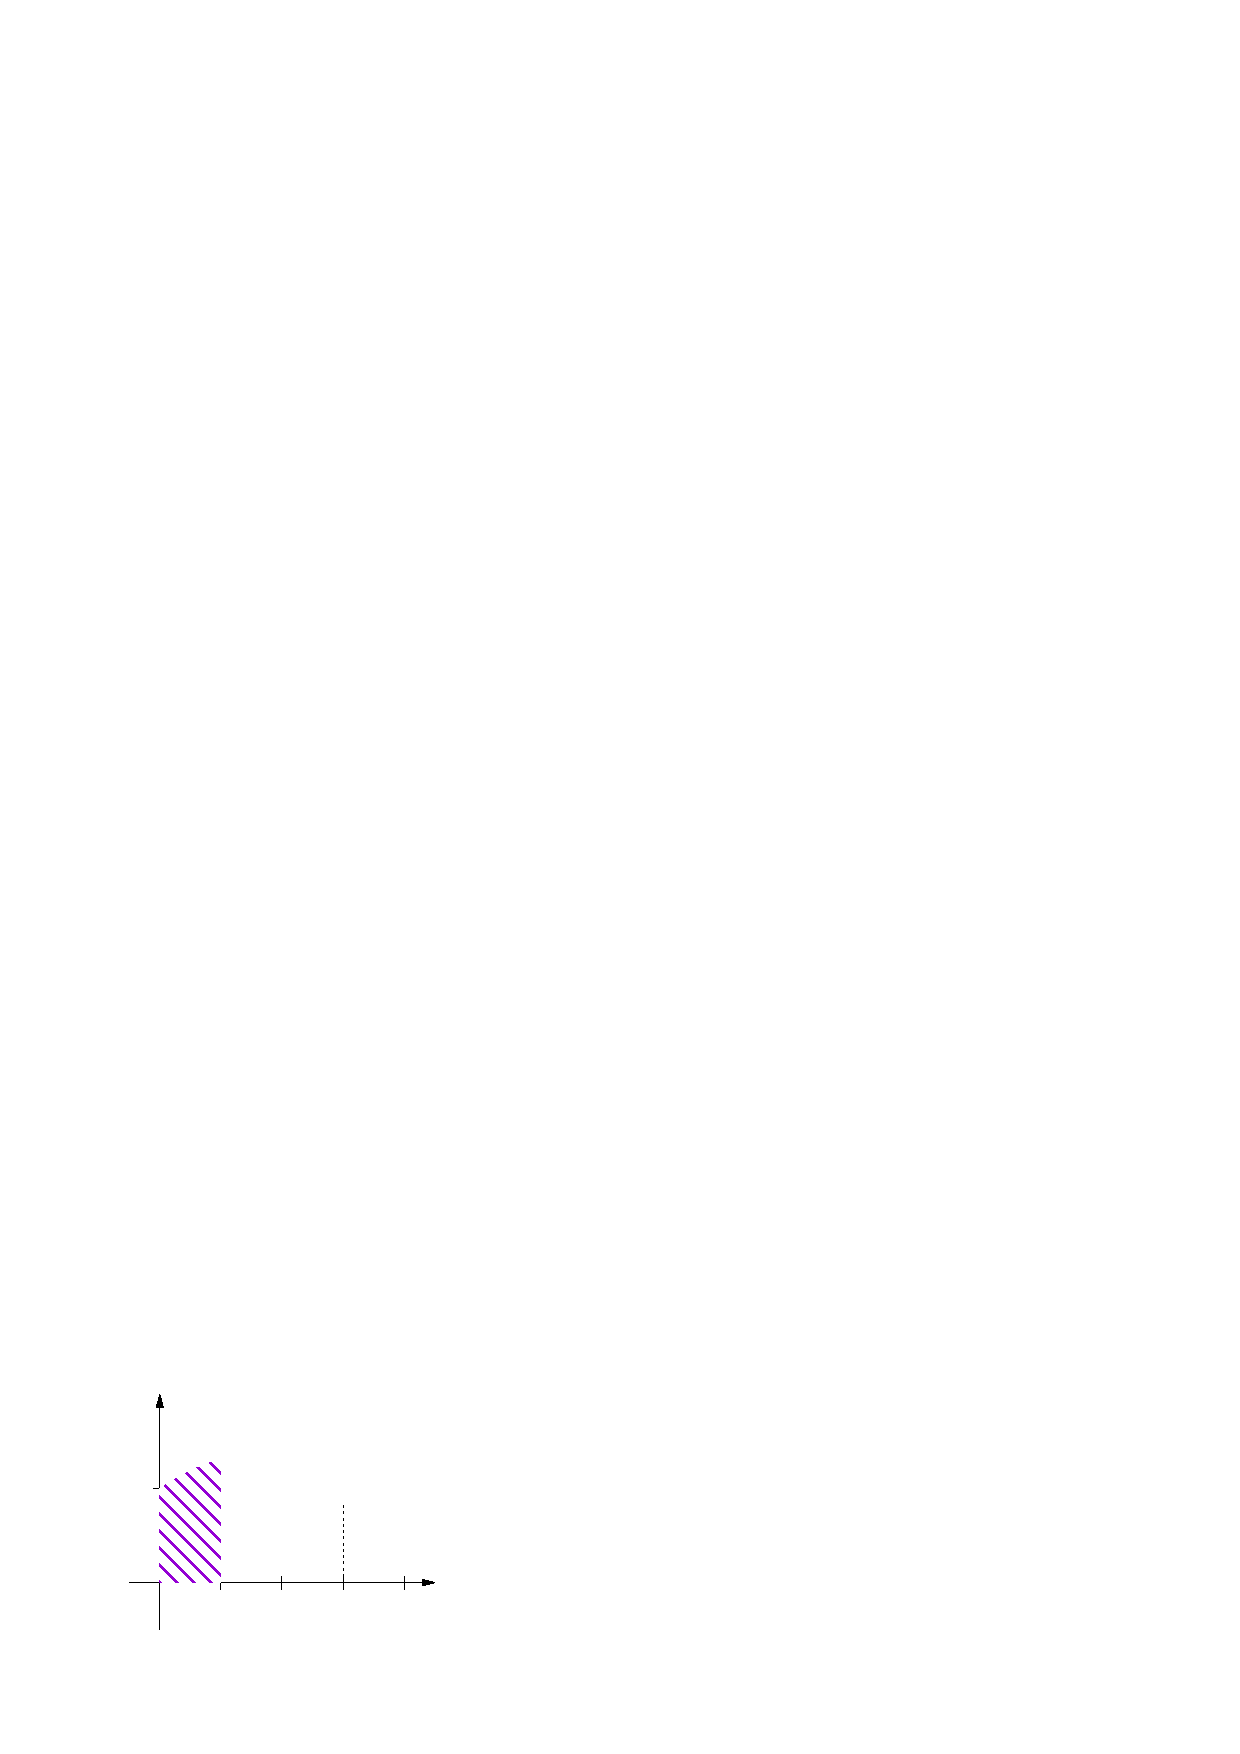
\includegraphics[width={158.40bp},height={108.00bp}]{figura_05_04}}%
    \gplfronttext
  \end{picture}%
\endgroup

    \end{minipage}
\end{figure}

\section{Transformada de \emph{Fourier} y convolución}
\begin{equation}
    \mathcal{F}\{f_1(t)*f_2(t)\}=F_1(\omega)\,F_2(\omega)
\end{equation}
Donde:
\begin{equation*}
    F_1(\omega)=\mathcal{F}\{f_1(t)\}
\end{equation*}
\begin{equation*}
    F_2(\omega)=\mathcal{F}\{f_2(t)\}
\end{equation*}

\underline{Prueba}:
\begin{equation*}
\begin{split}
    \mathcal{F}\{f_1(t)*f_2(t)\}
        &=\int_{-\infty}^{\infty}\left[
            \int_{\infty}^{\infty}f_1(\tau)f_2(t-\tau)d\tau
        \right]\,e^{-jn\omega_0\,t}\,dt\\
        &=\int_{-\infty}^{\infty}\int_{-\infty}^{\infty}
            f_1(\tau)f_2(t-\tau)\,e^{-jn\omega_0\,t}\,d\tau\,dt\\
        &=\int_{-\infty}^{\infty}\int_{-\infty}^{\infty}
            f_1(\tau)f_2(t-\tau)\,e^{-jn\omega_0\,t}\,dt\,d\tau\\
        &=\int_{-\infty}^{\infty}f_1(\tau)d\tau\,\int_{-\infty}^{\infty}
            f_2(t-\tau)\,e^{-jn\omega_0\,t}\,dt\\
\end{split}
\end{equation*}
\begin{equation*}
    u=t-\tau\rightarrow\,t=u+\tau
\end{equation*}
\begin{equation*}
    du=dt
\end{equation*}
\begin{equation*}
\begin{split}
    \mathcal{F}\{f_1(t)*f_2(t)\}
        &=\int_{-\infty}^{\infty}f_1(\tau)d\tau\,\int_{-\infty}^{\infty}
            f_2(u)\,e^{-jn\omega_0(u+\tau)}\,du\\
        &=\int_{-\infty}^{\infty}f_1(\tau)\,e^{-jn\omega_0\tau}\,d\tau\,
            \int_{-\infty}^{\infty}f_2(u)\,e^{-jn\omega_0\,u}\,du\\
        &=F_1(\omega)\,F_2(\omega)\\
\end{split}
\end{equation*}

\section{Transformada inversa de \emph{Fourier} por convolución}
\begin{equation}
    \mathcal{F}^{-1}\{F_1(\omega)\,F_2(\omega)\}=f_1(t)*f_2(t)
\end{equation}
Donde:
\begin{equation*}
    f_1(t)=\mathcal{F}^{-1}\{F_1(\omega)\}
\end{equation*}
\begin{equation*}
    f_2(t)=\mathcal{F}^{-1}\{F_2(\omega)\}
\end{equation*}

\section{Ecuaciones diferenciales ordinarias}
\begin{equation*}
    \mathcal{F}\{f'(t)\}=j\omega\,F(\omega)
\end{equation*}
\begin{equation*}
    \mathcal{F}\{f''(t)\}={(j\omega)}^2\,F(\omega)
\end{equation*}
\begin{equation*}
    \mathcal{F}\{f^{(n)}(t)\}={(j\omega)}^n\,F(\omega)
\end{equation*}

